\section{Pendahuluan}
Berisi deskripsi awal praktikum yang dilakukan pada hari itu
%===========================================================%
\section{Tujuan Praktikum}
Tujuannya apa kamu melakukan praktikum ini
%===========================================================%
\section{Alat dan Bahan}
\begin{itemize}[label=$\bullet$, itemsep=-1pt, leftmargin=*]
	\item paham lah ya isinya
\end{itemize}
%===========================================================%
\section{Langkah-langkah Percobaan}

\subsection{Judul Percobaan 1}
\begin{enumerate}
	\item Konfigurasi router1 dengan ip address 123.656.78.1/24
	\begin{figure}[H]
		\centering
		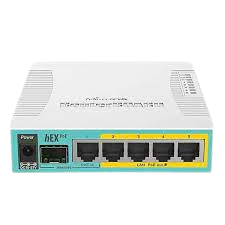
\includegraphics[width=0.5\linewidth]{P1/img/contoh.png}
		\caption{Gambar Contoh}
		\label{fig:gambar1}
	\end{figure}
\end{enumerate}

\subsection{Judul Percobaan 2}
\begin{enumerate}
	\item 
\end{enumerate}
%===========================================================%
\section{Hasil Percobaan}
Hasil dari percobaan yang sudah kamu buat
%===========================================================%
\section{Kesimpulan}
simpulkan
%===========================================================%
\section{Lampiran}
berisi tugas pendahuluan dan dokumentasi saat melakukan praktikum